\documentclass[10pt]{beamer}
\usetheme{Frankfurt}
\usepackage[utf8]{inputenc}
\usepackage[spanish,es-tabla]{babel}
%\usepackage[T1]{fontenc}
\usepackage{amsmath}
\usepackage{amsfonts}
\usepackage{amssymb}
\usepackage{graphicx}
\graphicspath{{imagenes/}}
\author{Ciro Fabián Bermúdez Márquez}
\title{TRNGs para generación de secuencias muy largas}
\institute{Instituto Nacional de Astrofísica, Óptica y Electrónica} 
\date{\today} 

%-------------------------------------------------------------------------------
%                            Paquetes adicionales                              %
%-------------------------------------------------------------------------------
%-------------------------------------------------------------------------------
%                                Paquetes extras                               %
%-------------------------------------------------------------------------------
\setcounter{secnumdepth}{3}
\setcounter{tocdepth}{3} 
\usepackage{amsthm}
\theoremstyle{definition}
\newtheorem{axiom}{Axioma} %[chapter]
\renewcommand\theaxiom{\Roman{axiom}}

\theoremstyle{definition}
\newtheorem{property}{Propiedad} %[chapter]

\theoremstyle{definition}
\newtheorem{corollary}{Corolario} %[chapter]

\theoremstyle{definition}
\newtheorem{theorem}{Teorema} %[chapter]

\usepackage{lipsum}												% Texto de ejemplo \lipsum[1-30]
\decimalpoint													% Punto decimal en lugar de coma
\spanishsignitems												% Viñetas en lugar de cuadros
\raggedbottom													% Eliminar molestos warnings

\usepackage{comment}											% Comentarios largos
\usepackage{pdfpages}											% Incluir portada echa en Inkscape
\usepackage{setspace}											% Interlineado
\usepackage{makecell}											% Para tablas
\usepackage{xcolor}												% Colores en tablas
\usepackage{colortbl}
\usepackage{multirow}
\usepackage{array}												% Necesario para algunas tablas
\usepackage[inline]{enumitem}									% Personalizar itemize
\usepackage{multicol}											% Item 2 columns

\definecolor{Red}{RGB}{255,191,191}								% Colores definidos por el usuario

\usepackage[nottoc]{tocbibind}									% Bibliografia en table of contents

\usepackage[figuresright]{rotating}								% Rotar figuras con caption
\usepackage{subcaption}											% Subfiguras
%-------------------------------------------------------------------------------
%                            Comandos matematicos                              %
%-------------------------------------------------------------------------------
\usepackage{steinmetz}											% Para representar fasores
\usepackage{bm}													% Bold math  \bm command
\newcommand{\binomb}[2]{\genfrac{[}{]}{0pt}{}{#1}{#2}}
%-------------------------------------------------------------------------------
%                        Paquetes para hipervinculos                           %
%-------------------------------------------------------------------------------
\usepackage[hidelinks]{hyperref}								% Añade los bookmarks y le quita la caja roja, \url{}
\urlstyle{same}
%-------------------------------------------------------------------------------
%                           Estilos de encabezados                             %
%-------------------------------------------------------------------------------
\usepackage{fancyhdr, blindtext}								% Libreria para encabezados

\renewcommand{\chaptermark}[1]{\markboth{#1}{}}					% Capitulos y secciones en minusculas
\renewcommand{\sectionmark}[1]{\markright{#1}}

\fancypagestyle{normalstyle}{%
  \fancyhf{}													% Reinicial estilos de header y footer
	\fancyhead[LE,RO]{\thepage}
	\fancyhead[LO]{\nouppercase{\rightmark}}
	\fancyhead[RE]{\nouppercase{\leftmark}}
	\renewcommand{\headrulewidth}{0.4pt}
	\renewcommand{\footrulewidth}{0pt}
	\setlength{\headheight}{14.62pt}
}

\fancypagestyle{Resumen}{%
  \fancyhf{}													% Reinicial estilos de header y footer
	\fancyhead[LE,RO]{\thepage}
	\fancyhead[LO]{\nouppercase{Resumen}}
	\fancyhead[RE]{\nouppercase{Resumen}}
	\renewcommand{\headrulewidth}{0.4pt}
	\renewcommand{\footrulewidth}{0pt}
	\setlength{\headheight}{14.62pt}
}
%-------------------------------------------------------------------------------
%                            Libreria de codigos                               %
%-------------------------------------------------------------------------------
% Paquetes necesarios
\usepackage{listings}
\usepackage{xcolor}

% Colores para tablas
\definecolor{Gray}{RGB}{230,230,230}
\definecolor{Red}{RGB}{255,191,191}

% Colores personalizados
\definecolor{verde}{rgb}{0,0.6,0}
\definecolor{gris}{RGB}{253, 253, 253}
\definecolor{grisfuerte}{RGB}{140, 140, 140}

% Deficion de lenguajes perzonalizados

% Estilos MATLAB
\lstdefinestyle{MATLAB}{
	language=MATLAB,
	basicstyle=\linespread{1}\tiny\fontfamily{pcr}\selectfont,
	backgroundcolor=\color{gris},
	frame=single,
	frameround=tttt,
	rulecolor=\color{black},
	commentstyle=\color{verde},
	keywordstyle=\color{blue}, %magenta
	stringstyle=\color{grisfuerte},                  
	captionpos=t,                    
	breaklines=true,                       
	breakatwhitespace=false,
	showspaces=false,                
	showstringspaces=false,
	showtabs=false,
	keepspaces=true,
	columns=flexible,
	tabsize=4,   
}

\lstdefinestyle{VHDL}{
	language=VHDL,
	basicstyle=\linespread{1}\tiny\fontfamily{pcr}\selectfont,
	backgroundcolor=\color{gris},
	frame=single,
	frameround=tttt,
	rulecolor=\color{black},
	commentstyle=\color{verde},
	keywordstyle=\color{blue}, %magenta
	stringstyle=\color{grisfuerte},                  
	captionpos=t,                    
	breaklines=true,                       
	breakatwhitespace=false,
	showspaces=false,                
	showstringspaces=false,
	showtabs=false,
	keepspaces=true,
	columns=flexible,
	tabsize=4,
	upquote=true,
}


\lstdefinestyle{VHDL_TEXT}{
	language=VHDL,
	basicstyle=\linespread{1}\footnotesize\fontfamily{pcr}\selectfont,
	backgroundcolor=\color{gris},
	frame=single,
	frameround=tttt,
	rulecolor=\color{black},
	commentstyle=\color{verde},
	keywordstyle=\color{blue}, %magenta
	stringstyle=\color{grisfuerte},                  
	captionpos=t,                    
	breaklines=true,                       
	breakatwhitespace=false,
	showspaces=false,                
	showstringspaces=false,
	showtabs=false,
	keepspaces=true,
	columns=flexible,
	tabsize=4,
	upquote=true,
}


\lstdefinestyle{C}{
	language=C,
	basicstyle=\linespread{1}\tiny\fontfamily{pcr}\selectfont,
	backgroundcolor=\color{gris},
	frame=single,
	frameround=tttt,
	rulecolor=\color{black},
	commentstyle=\color{verde},
	keywordstyle=\color{blue}, %magenta
	stringstyle=\color{grisfuerte},                  
	captionpos=t,                    
	breaklines=true,                       
	breakatwhitespace=false,
	showspaces=false,                
	showstringspaces=false,
	showtabs=false,
	keepspaces=true,
	columns=flexible,
	tabsize=4,
	upquote=true,    
}

\renewcommand{\lstlistingname}{Código}% Listing -> Algorithm
\renewcommand{\lstlistlistingname}{Lista de códigos}% 

%-------------------------------------------------------------------------------
%                           Caption en negritas                                %
%-------------------------------------------------------------------------------
\usepackage[labelfont=bf]{caption}
\captionsetup{labelfont=bf}


%-------------------------------------------------------------------------------
%                           Lista de conceptos                                %
%-------------------------------------------------------------------------------
\usepackage[nonumberlist,nogroupskip,toc,style=super]{glossaries}
\setlength{\glsdescwidth}{0.7\textwidth}

\makeglossaries

\newglossaryentry{FPGA}
{
    name=FPGA, %% $\qquad\qquad\qquad\qquad$
    description={Field Programmable Logic Array}
}

\newglossaryentry{RNG}
{
    name=RNG,
    description={Random Number Generator}
}

\newglossaryentry{TRNG}
{
    name=TRNG,
    description={True Random Number Generator}
}

\newglossaryentry{TERO}
{
    name=TERO,
    description={Transient Effect Ring Oscillator}
}

\newglossaryentry{ERO-TRNG}
{
    name=ERO-TRNG,
    description={Elementary ring oscillator based TRNG}
}

\newglossaryentry{COSO-TRNG}
{
    name=COSO-TRNG,
    description={Coherent sampling ring oscillator based TRNG}
}

\newglossaryentry{MURO-TRNG}
{
    name=MURO-TRNG,
    description={Multi-ring oscillator based TRNG}
}


\newglossaryentry{TERO-TRNG}
{
    name=TERO-TRNG,
    description={Transient effect ring oscillator based TRNG}
}

\newglossaryentry{PLL-TRNG}
{
    name=PLL-TRNG,
    description={Phase-locked loop based TRNG}
}


\newglossaryentry{STR-TRNG}
{
    name=STR-TRNG,
    description={Self-timed ring based TRNG}
}




\begin{document}

% Slide
\begin{frame}[plain]
    \fontfamily{cmr}\selectfont
	\begin{center}
		\textbf{Instituto Nacional de Astrofísica, Óptica y Electrónica (INAOE)}
	\end{center}
	
	\begin{figure}[hbtp]
		\centering
		
\includegraphics[width = 2cm]{Inaoe} 
	\end{figure}
	
	\begin{center}
		Maestría en Ciencias en Electrónica
	\end{center}
					
	\begin{center}
		\begin{Large}
		\textcolor{blue}{TRNGs para generación de secuencias muy largas}
		\end{Large}
	\end{center}
	
	\begin{center}
		\textbf{Autor:} Ciro Fabián Bermúdez Márquez
	\end{center}
	
	\begin{flushleft}
		\textbf{Asesor:} Dr. Esteban Tlelo Cuautle (INAOE)\\
	    \textbf{Coasesor:} Dr. Cuauhtemoc Mancillas López (CINVESTAV IPN)
	\end{flushleft}
	
	\begin{flushright}
	    \today
	\end{flushright}
\end{frame}

% Slide
\begin{frame}
    \tableofcontents
\end{frame}

% Slide
\section{Introducción}


% Slide
\begin{frame}
    \frametitle{Introducción}
    \begin{block}{}
        \justifying
	\end{block}
\end{frame}



% Slide
\section{Objetivos}
\begin{frame}
    \frametitle{Objetivos}
    \begin{block}{Objetivo general}
        \justifying
        Diseñar e implementar en FPGA un TRNG híbrido para la generación de secuencias muy largas.
	\end{block}

    \begin{block}{Objetivo específicos}
        \justifying
        \begin{itemize}
            \item[•] Investigar el estado del arte de diferentes generadores de números aleatorios.
            \item[•] Estudiar los diferentes tipos de generadores de números aleatorios y analizar sus características principales.
            \item[•] Estudiar la teoría de los mapas caóticos y su utilidad en generadores de números aleatorios.
            \item[•] Diseñar un generador de números aleatorios híbrido utilizando un TRNG como generador de semillas y un mapa caótico para realizar un postprocesamiento que mejore sus características estadísticas y comprobar estas utilizando las pruebas NIST.
            \item[•] Implementar el TRNG híbrido en una FPGA.
        \end{itemize}
	\end{block}

\end{frame}

% Slide 
\section{Generadores de números aleatorios (RNGs)}
\begin{frame}
    \frametitle{Introducción}
    \begin{block}{Estructura de los TRNG}
        \justifying
        Lorem ipsum dolor sit amet, consectetur adipiscing elit. Aenean lobortis fermentum arcu, in pretium risus convallis vel. Aenean dignissim quis felis.
	\end{block}
	
	\begin{figure}[hbtp]
	    \centering
	    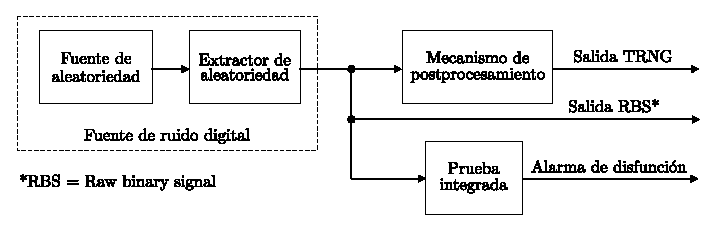
\includegraphics[width=0.8\textwidth]{A0_TRNG_estructura}
	    \caption{Estructura general de un TRNG \cite{Badrignans2011}.}
        \label{fig:A1_TRNG_estructura}
    \end{figure}
\end{frame}

% Slide
\begin{frame}
    \frametitle{Introducción}
    \begin{block}{Parámetros de evaluación}
        \justifying
		\begin{itemize}
		    \item Parámetros relacionados con la calidad
		        \begin{itemize}
		            \item Fuente de aleatoriedad.
		            \item Método de extracción de aleatoriedad y entropía del ruido digital.
		            \item Método de postprocesamiento (opcional).
		            \item Tasa de bits de salida y su estabilidad.
		        \end{itemize}
		    \item Parámetros relacionados con la seguridad
		        \begin{itemize}
		            \item Existencia de un modelo matemático.
		            \item Comprobabilidad interna.
		            \item Seguridad (robustez, resistencia contra ataques).
		        \end{itemize}
		    \item Parámetros relacionados con el diseño
		        \begin{itemize}
		            \item El uso de recursos.
		            \item El consumo de energía.
		            \item Viabilidad en dispositivos lógicos y FPGAs.
		            \item Automatización del diseño.
		        \end{itemize}
		\end{itemize}   
		\vspace{0.1cm}
	\end{block}
\end{frame}


% Slide
\begin{frame}
    \frametitle{Introducción}
    \begin{block}{Jitter}
        \justifying
         Lorem ipsum dolor sit amet, consectetur adipiscing elit. Aenean lobortis fermentum arcu, in pretium risus convallis vel. Aenean dignissim quis felis. 
	\end{block}
	\begin{figure}[hbtp]
        \centering
        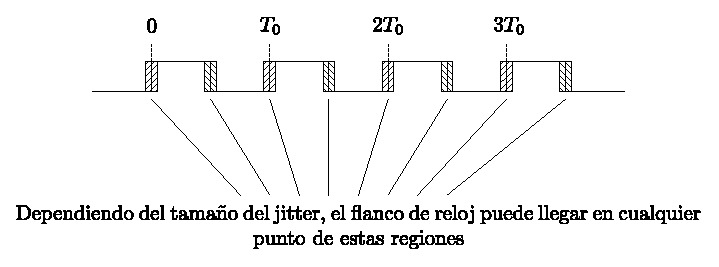
\includegraphics[width=0.8\textwidth]{F9_jitter}
        \caption{Jitter del reloj.}
        \label{fig:F9_jitter}
    \end{figure}
\end{frame}


% Slide
\begin{frame}
    \frametitle{Introducción}
    \begin{block}{Jitter}
        \justifying
         Lorem ipsum dolor sit amet, consectetur adipiscing elit. Aenean lobortis fermentum arcu, in pretium risus convallis vel. Aenean dignissim quis felis.
	\end{block}
    \begin{figure}[hbtp]
        \centering
        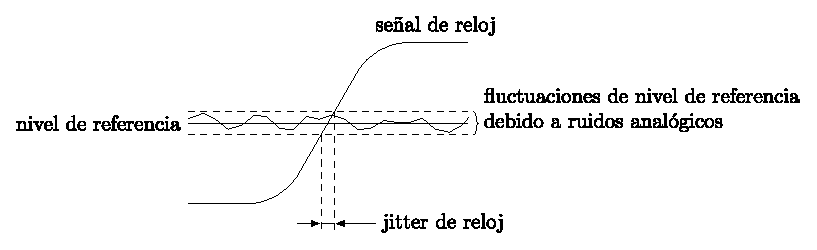
\includegraphics[width=0.8\textwidth]{F10_fluctuaciones}
        \caption{Fluctuaciones del nivel de referencia originadas por ruidos analógicos que provocan jitter del reloj en los circuitos digitales. \cite{Petura2019}}
        \label{fig:F10_fluctuaciones}
    \end{figure}
\end{frame}



% Slide
\begin{frame}
    \frametitle{Introducción}
    \begin{block}{Núcleos TRNG en FPGA}
        \justifying
        Con base en los criterios del AIS-20/31 \cite{Petura2016}, los núcleos TRNG adecuados para utilizarse en dispositivos lógicos programables (FPGA) que usan estructuras oscilantes son:
		\begin{itemize}
            \item Elementary ring oscillator based TRNG (ERO-TRNG).
            \item Coherent sampling ring oscillator based TRNG (COSO-TRNG).
            \item Multi-ring oscillator based TRNG (MURO-TRNG).
            \item Transient effect ring oscillator based TRNG (TERO-TRNG).
            \item Self-timed ring based TRNG  (STR-TRNG).
            \item Phase-locked loop based TRNG (PLL-TRNG).
        \end{itemize}  
	\end{block}
\end{frame}


% Slide
\begin{frame}
    \frametitle{Introducción}
    \begin{block}{Núcleo ERO-TRNG}
        \justifying
         Lorem ipsum dolor sit amet, consectetur adipiscing elit. Aenean lobortis fermentum arcu, in pretium risus convallis vel. Aenean dignissim quis felis interdum aliquam. Duis et vehicula nulla.   
	\end{block}
	\begin{figure}[hbtp]
	    \centering
	    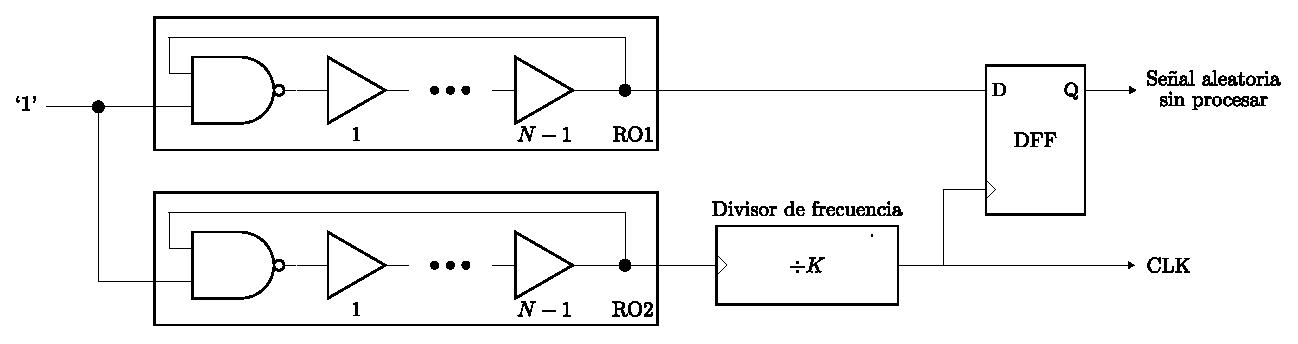
\includegraphics[width=0.8\textwidth]{A1_ERO_TRNG}
	    \caption{Diagrama de ERO-TRNG.}
        \label{fig:A1_ERO_TRNG}
    \end{figure}
\end{frame}

% Slide
\begin{frame}
    \frametitle{Introducción}
    \begin{block}{Núcleo COSO-TRNG}
        \justifying
         Lorem ipsum dolor sit amet, consectetur adipiscing elit. Aenean lobortis fermentum arcu, in pretium risus convallis vel. Aenean dignissim quis felis interdum aliquam. Duis et vehicula nulla.   
	\end{block}
	\begin{figure}[hbtp]
	    \centering
	    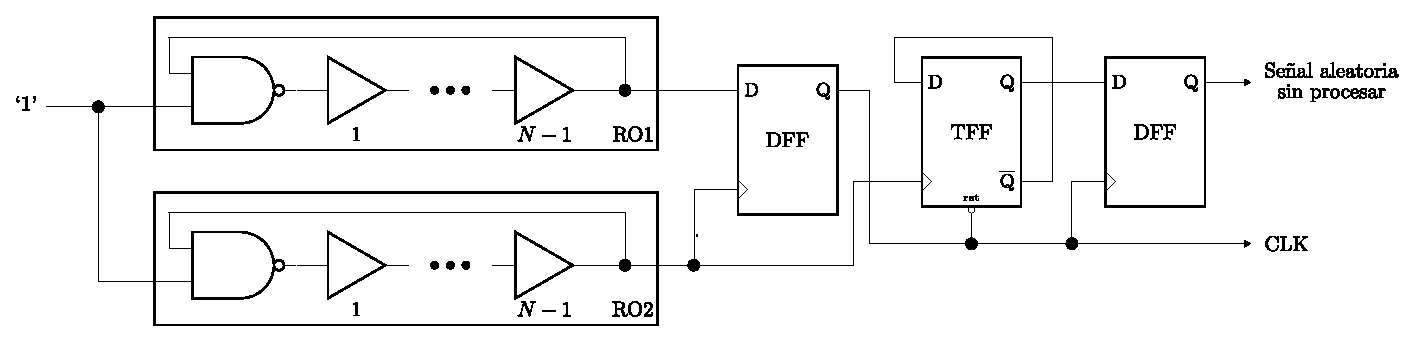
\includegraphics[width=0.8\textwidth]{A2_COSO_TRNG}
	    \caption{Diagrama de COSO-TRNG.}
        \label{fig:A2_COSO_TRNG}
    \end{figure}
\end{frame}


% Slide
\begin{frame}
    \frametitle{Introducción}
    \begin{block}{Núcleo MURO-TRNG}
        \justifying
         Lorem ipsum dolor sit amet, consectetur adipiscing elit. Aenean lobortis fermentum arcu, in pretium risus convallis vel. Aenean dignissim quis felis interdum aliquam. Duis et vehicula nulla.   
	\end{block}
	\begin{figure}[hbtp]
	    \centering
	    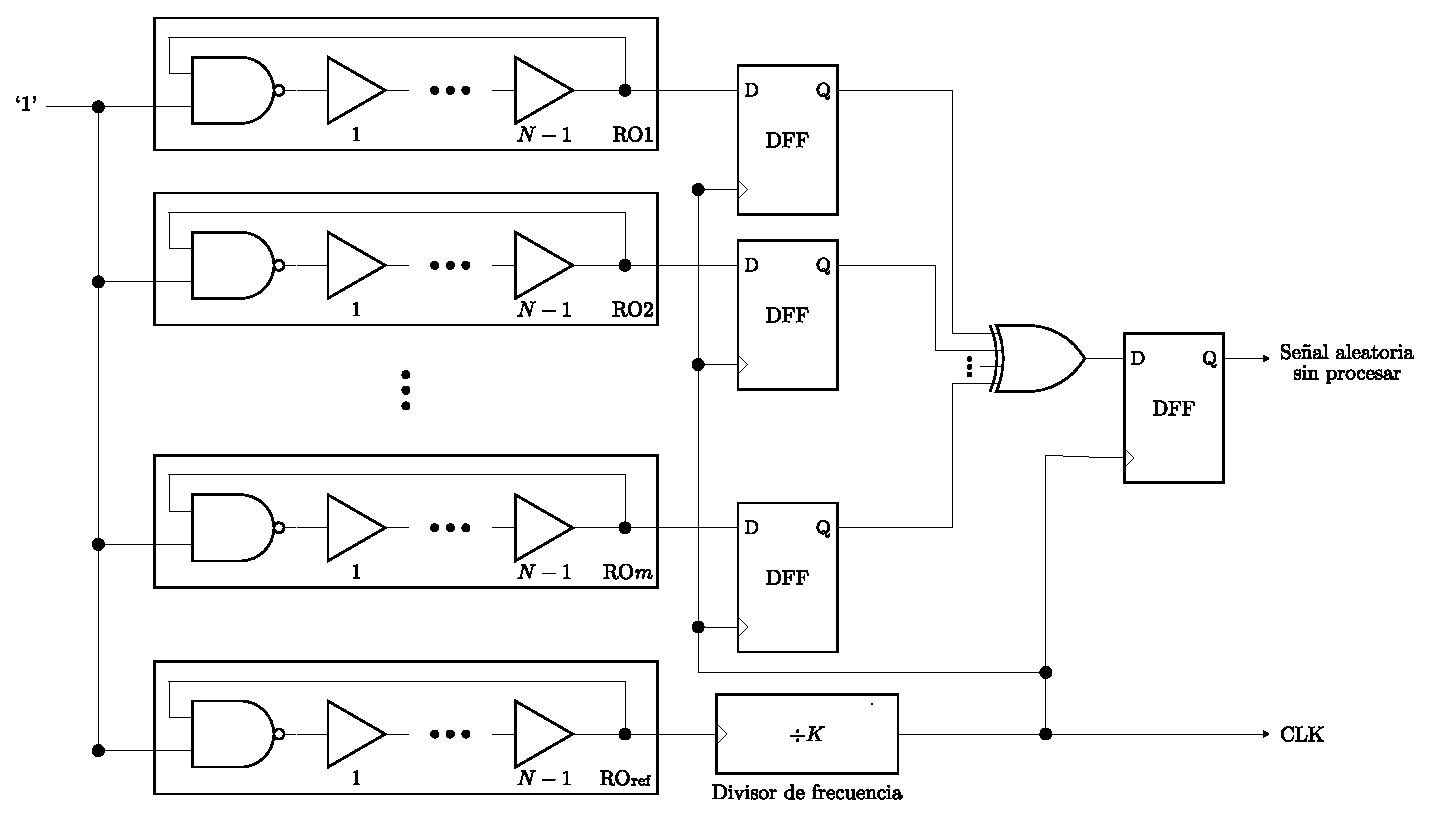
\includegraphics[width=0.6\textwidth]{A3_MURO_TRNG}
	    \caption{Diagrama de MURO-TRNG.}
        \label{fig:A3_MURO_TRNG}
    \end{figure}
\end{frame}


% Slide
\begin{frame}
    \frametitle{Introducción}
    \begin{block}{Núcleo TERO-TRNG}
        \justifying
         Lorem ipsum dolor sit amet, consectetur adipiscing elit. Aenean lobortis fermentum arcu, in pretium risus convallis vel. Aenean dignissim quis felis interdum aliquam. Duis et vehicula nulla.   
	\end{block}
	\begin{figure}[hbtp]
	    \centering
	    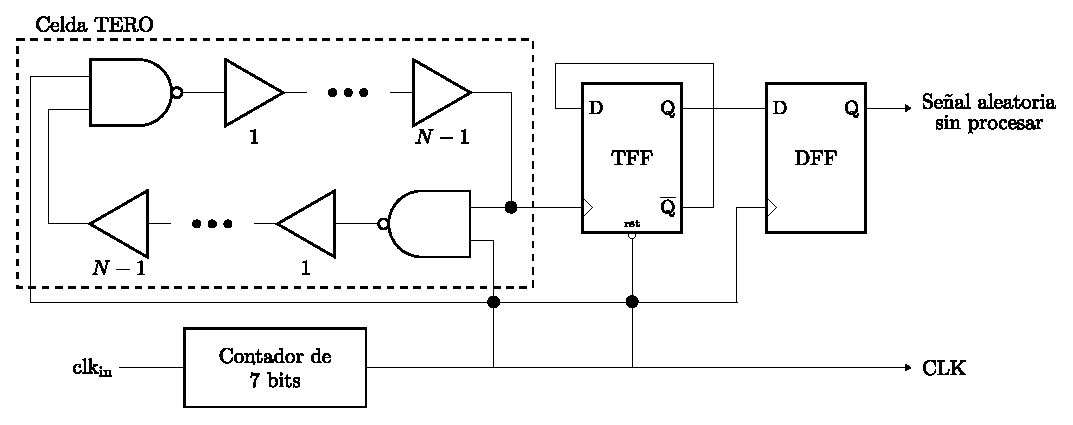
\includegraphics[width=0.6\textwidth]{A4_TERO_TRNG}
	    \caption{Diagrama de TERO-TRNG.}
        \label{fig:A4_TERO_TRNG}
    \end{figure}
\end{frame}


% Slide
\begin{frame}
    \frametitle{Introducción}
    \begin{block}{Núcleo STR-TRNG}
        \justifying
         Lorem ipsum dolor sit amet, consectetur adipiscing elit. Aenean lobortis fermentum arcu, in pretium risus convallis vel. Aenean dignissim quis felis interdum aliquam. Duis et vehicula nulla.   
	\end{block}
	\begin{figure}[hbtp]
	    \centering
	    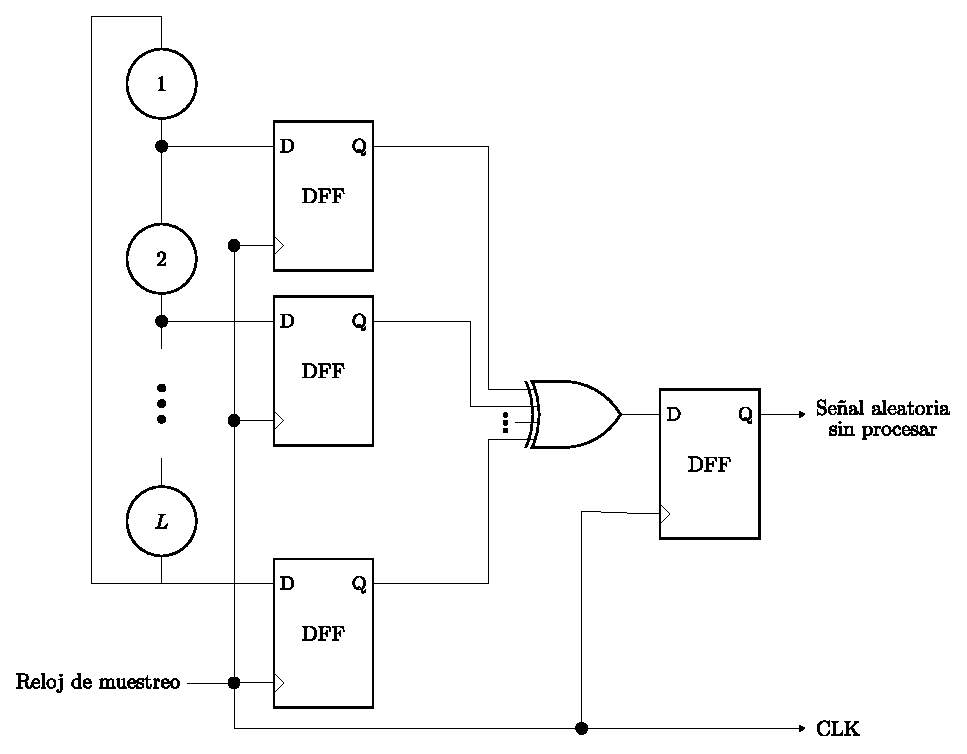
\includegraphics[width=0.5\textwidth]{A5_STR_TRNG}
	    \caption{Diagrama de STR-TRNG.}
        \label{fig:A5_STR_TRNG}
    \end{figure}
\end{frame}


% Slide
\begin{frame}
    \frametitle{Introducción}
    \begin{block}{Núcleo PLL-TRNG}
        \justifying
         Lorem ipsum dolor sit amet, consectetur adipiscing elit. Aenean lobortis fermentum arcu, in pretium risus convallis vel. Aenean dignissim quis felis interdum aliquam. Duis et vehicula nulla.   
	\end{block}
	\begin{figure}[hbtp]
	    \centering
	    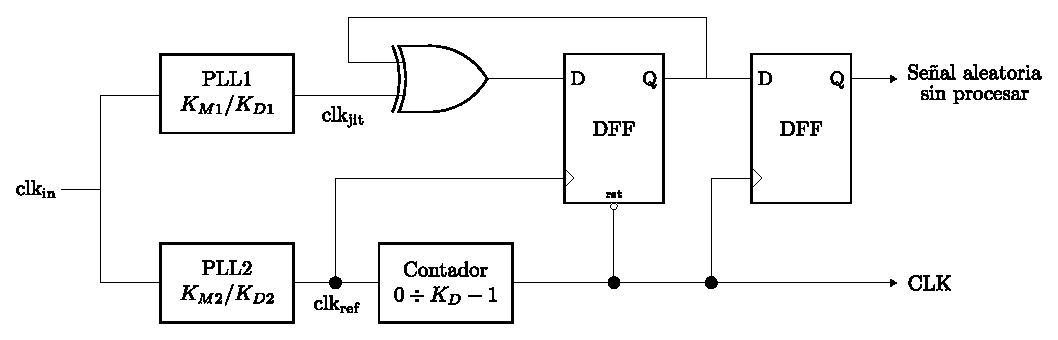
\includegraphics[width=0.7\textwidth]{A6_PLL_TRNG}
	    \caption{Diagrama de PLL-TRNG.}
        \label{fig:A6_PLL_TRNG}
    \end{figure}
\end{frame}


% Slide
\begin{frame}
    \frametitle{Introducción}
    \begin{block}{Núcleos TRNG en FPGA}
        \justifying
\begin{table}[htbp]
  \centering
    \caption{Resumen de los resultados núcleos TRNGs \cite{Petura2016}.}
    \resizebox{0.9\linewidth}{!}{ 
        \begin{tabular}{|c|c|c|c|c|c|c|c|c|}
            \hline
            \rowcolor{lightgray} TRNG Type & FPGA  & Area  & Power cons. & Bit Rate & Efficiency & Entropy & Entropy * Bit rate & Feasib. \\
            \rowcolor{lightgray}       & device & (LUT/Reg) & [mW]  & [Mbits/s] & [bits/$\mu$Ws] & per bit &       & \& Repeat. \\
            \hline
            \multirow{3}[2]{*}{ERO} & Spartan 6 & 46/19 & 2.16  & 0.0042 & 1.94  & 0.999 & 0.004 & \multirow{3}[2]{*}{5} \\
                  & Cyclone V & 34/20 & 3.24  & 0.0027 & 0.83  & 0.990 & 0.003 &  \\
                  & SmartFusion 2 & 45/19 & 4     & 0.014 & 3.5   & 0.980 & 0.013 &  \\
            \hline
            \multirow{3}[2]{*}{COSO} & Spartan 6 & 18/3  & 1.22  & 0.54  & 442.6 & 0.999 & 0.539 & \multirow{3}[2]{*}{1} \\
                  & Cyclone V & 13/3  & 0.9   & 1.44  & 1600  & 0.999 & 1.438 &  \\
                  & SmartFusion 2 & 23/3  & 1.94  & 0.328 & 169   & 0.999 & 0.327 &  \\
            \hline
            \multirow{3}[2]{*}{MURO} & Spartan 6 & 521/131 & 54.72 & 2.57  & 46.9  & 0.999 & 2.567 & \multirow{3}[2]{*}{4} \\
                  & Cyclone V & 525/130 & 34.93 & 2.2   & 62.9  & 0.999 & 2.197 &  \\
                  & SmartFusion 2 & 545/130 & 66.41 & 3.62  & 54.5  & 0.999 & 3.616 &  \\
            \hline
            \multirow{3}[2]{*}{PLL} & Spartan 6 & 34/14 & 10.6  & 0.44  & 41.5  & 0.981 & 0.431 & \multirow{3}[2]{*}{3} \\
                  & Cyclone V & 24/14 & 23    & 0.6   & 43.4  & 0.986 & 0.592 &  \\
                  & SmartFusion 2 & 30/15 & 19.7  & 0.37  & 18.7  & 0.921 & 0.340 &  \\
            \hline
            \multirow{3}[2]{*}{TERO} & Spartan 6 & 39/12 & 3.312 & 0.625 & 188.7 & 0.999 & 0.624 & \multirow{3}[2]{*}{1} \\
                  & Cyclone V & 46/12 & 9.36  & 1     & 106.8 & 0.987 & 0.985 &  \\
                  & SmartFusion 2 & 46/12 & 1.23  & 1     & 813   & 0.999 & 0.999 &  \\
            \hline
            \multirow{3}[2]{*}{STR} & Spartan 6 & 346/256 & 65.9  & 154   & 2343.2 & 0.998 & 154.121 & \multirow{3}[2]{*}{2} \\
                  & Cyclone V & 352/256 & 49.4  & 245   & 4959.1 & 0.999 & 244.755 &  \\
                  & SmartFusion 2 & 350/256 & 82.52 & 188   & 2286.7 & 0.999 & 188.522 &  \\
            \hline
        \end{tabular}%
    }
  \label{tab:resumen_de_trng_cores}
\end{table}%
   
	\end{block}
\end{frame}


% Slide
\section{Diseño de TRG híbrido}
\begin{frame}
    \frametitle{Título de diapositiva}
    \begin{block}{Título de bloque}
        \justifying
        \begin{equation}
        \begin{array}{ccl}
		    x_{n+1} & = &  a_{1} + a_{2}x_{n} + a_{3}x_{n}^{2} + a_{4}x_{n}y_{n} + a_{5}y_{n} + a_{6}y_{n}^{2}\\
		    y_{n+1} & = &  a_{7} + a_{8}x_{n} + a_{9}x_{n}^{2} + a_{10}x_{n}y_{n} + a_{11}y_{n} + a_{12}y_{n}^{2}
		\end{array}
	    \end{equation}
	\end{block}
\end{frame}


% Slide
\section{Bibliografía}
\begin{frame}
    \frametitle{Bibliografía}
    %\nocite{*}
	\bibliographystyle{ieeetr}
	\bibliography{../bibliografia}
\end{frame}


\end{document}
